\subsection{Homework 1 - Due: 09/04}\label{homework-1---due-0904}

\subsubsection{Problem 1}\label{problem-1}

Determine conclusively which of the following are fields:

\begin{enumerate}
\def\labelenumi{\alph{enumi}.}
\tightlist
\item
  The set of integers.
\item
  The set of rational numbers.
\item
  The set of polynomials of degree less than 3 with real coefficients.
\item
  The set of all \(n \times n\) matrices.
\item
  The set \(\{0,1\}\) with addition being binary ``exclusive-or'' and
  multiplication being binary ``and''.
\end{enumerate}

\subsubsection{Problem 2}\label{problem-2}

\begin{enumerate}
\def\labelenumi{\alph{enumi}.}
\tightlist
\item
  Define rules of addition and multiplication such that the set
  consisting of three elements \(\{a, b, c\}\) forms a field. Be sure to
  define the zero and unit elements.
\item
  Do Exercise 1 from Lecture Note 2 -
  \href{/exlecs/lec02.html\#exr-integersmodp}{Link}
\end{enumerate}

\subsubsection{Problem 3}\label{problem-3}

\begin{enumerate}
\def\labelenumi{\alph{enumi}.}
\tightlist
\item
  Let \(A\) be the linear operator in the plane denoting
  counter-clockwise rotation around the origin by some given angle
  \(\theta\). Compute the matrix of \(A\) relative to the standard basis
  in \(\mathbb{R}^2\).
\item
  Is the set \(\{I, A\}\) linearly dependent or independent in
  \(\left(\mathbb{R}^{2 \times 2}, \mathbb{R}\right)\) with
  \[ A = \begin{bmatrix} 1 & 1 \\ 0 & 2 \end{bmatrix} \]
\item
  What about the set \(\{I, A, A^2\}\)?
\end{enumerate}

\subsubsection{Problem 4}\label{problem-4}

Consider the standard double mass-spring-damper system. Derive the
equations of motion and put them in state space form:

\[ \dot{x} = A x + B u \]

where \[
x = \begin{bmatrix} p_1 & \dot{p}_1 & p_2 & \dot{p}_2 \end{bmatrix}^{T},
\]

is the state vector.

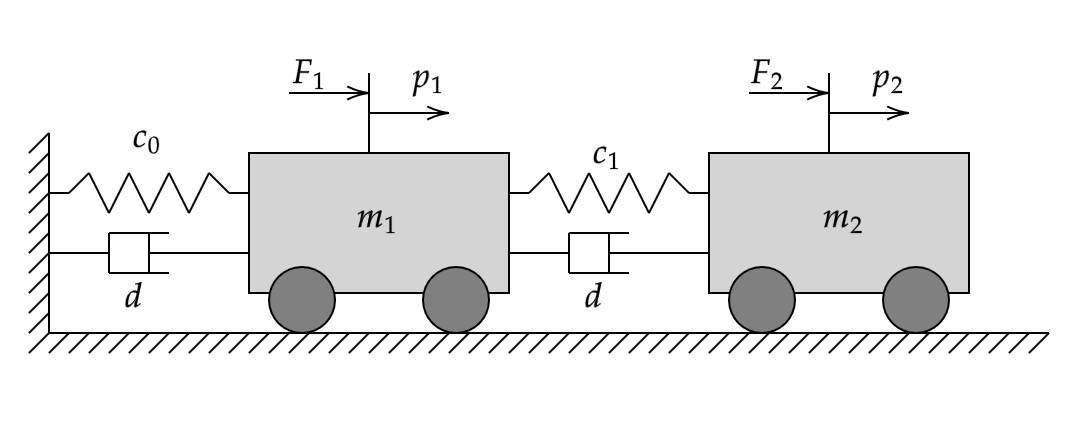
\includegraphics[width=0.5\linewidth,height=\textheight,keepaspectratio]{./figures/hw1_fig2.png}

\subsubsection{Problem 5}\label{problem-5}

Consider the standard RLC circuit, except now allow its characteristics
\(R, L\) and \(C\) to vary with time. Starting with the same non-dynamic
physical laws as in class (\(q = CV_c\) for the capacitor charge,
\(\varphi = LI\) for the inductor flux), derive a dynamical model of
this circuit. It should take the form:

\[ \dot{x} = A(t) x + B(t) u \]

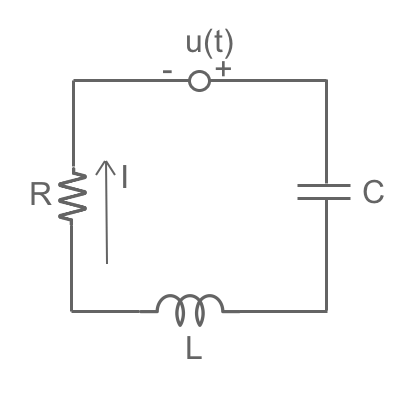
\includegraphics[width=0.3\linewidth,height=\textheight,keepaspectratio]{./figures/hw1_fig1.png}

\subsubsection{Problem 6}\label{problem-6}

\begin{enumerate}
\def\labelenumi{\alph{enumi}.}
\tightlist
\item
  Let \(S\) be the set of all vectors in \(\mathbb{R}^n\) whose
  components sum to zero. Prove that \(S\) is a subspace of
  \(\mathbb{R}^n\). Determine a basis for \(S\) and compute its
  dimension.
\item
  Provide a basis for the kernel of the linear operator \(L\) defined
  as:
\end{enumerate}

\begin{align*}
    L: \mathbb{R}^3 &\to \mathbb{R}^2 \\

  \left(x_1, x_2, x_3\right)^{T} &\mapsto \left(x_1 + 2x_2, x_2 - x_3\right)^T
  \end{align*}
